\documentclass[letterpaper,10pt,titlepage]{article}

\usepackage{graphicx}

\usepackage{amssymb}
\usepackage{amsmath}
\usepackage{amsthm}

\usepackage{alltt}
\usepackage{float}
\usepackage{color}
\usepackage{verbatim}

\usepackage{geometry}
\geometry{textheight=10in, textwidth=7.5in}

\usepackage{hyperref}

\def\name{Jordan Bayles (baylesj)}

%pull in the necessary preamble matter for pygments output
\input{pygments.tex}

%% The following metadata will show up in the PDF properties
\hypersetup{
  colorlinks = true,
  urlcolor = black,
  pdfauthor = {\name},
  pdfkeywords = {cs311 ``operating systems'' files filesystem I/O},
  pdftitle = {CS 311 Project 3: UNIX Process Control},
  pdfsubject = {CS 311 Project 3},
  pdfpagemode = UseNone
}

\parindent = 0.0 in
\parskip = 0.2 in

\begin{document}
\section{System design}
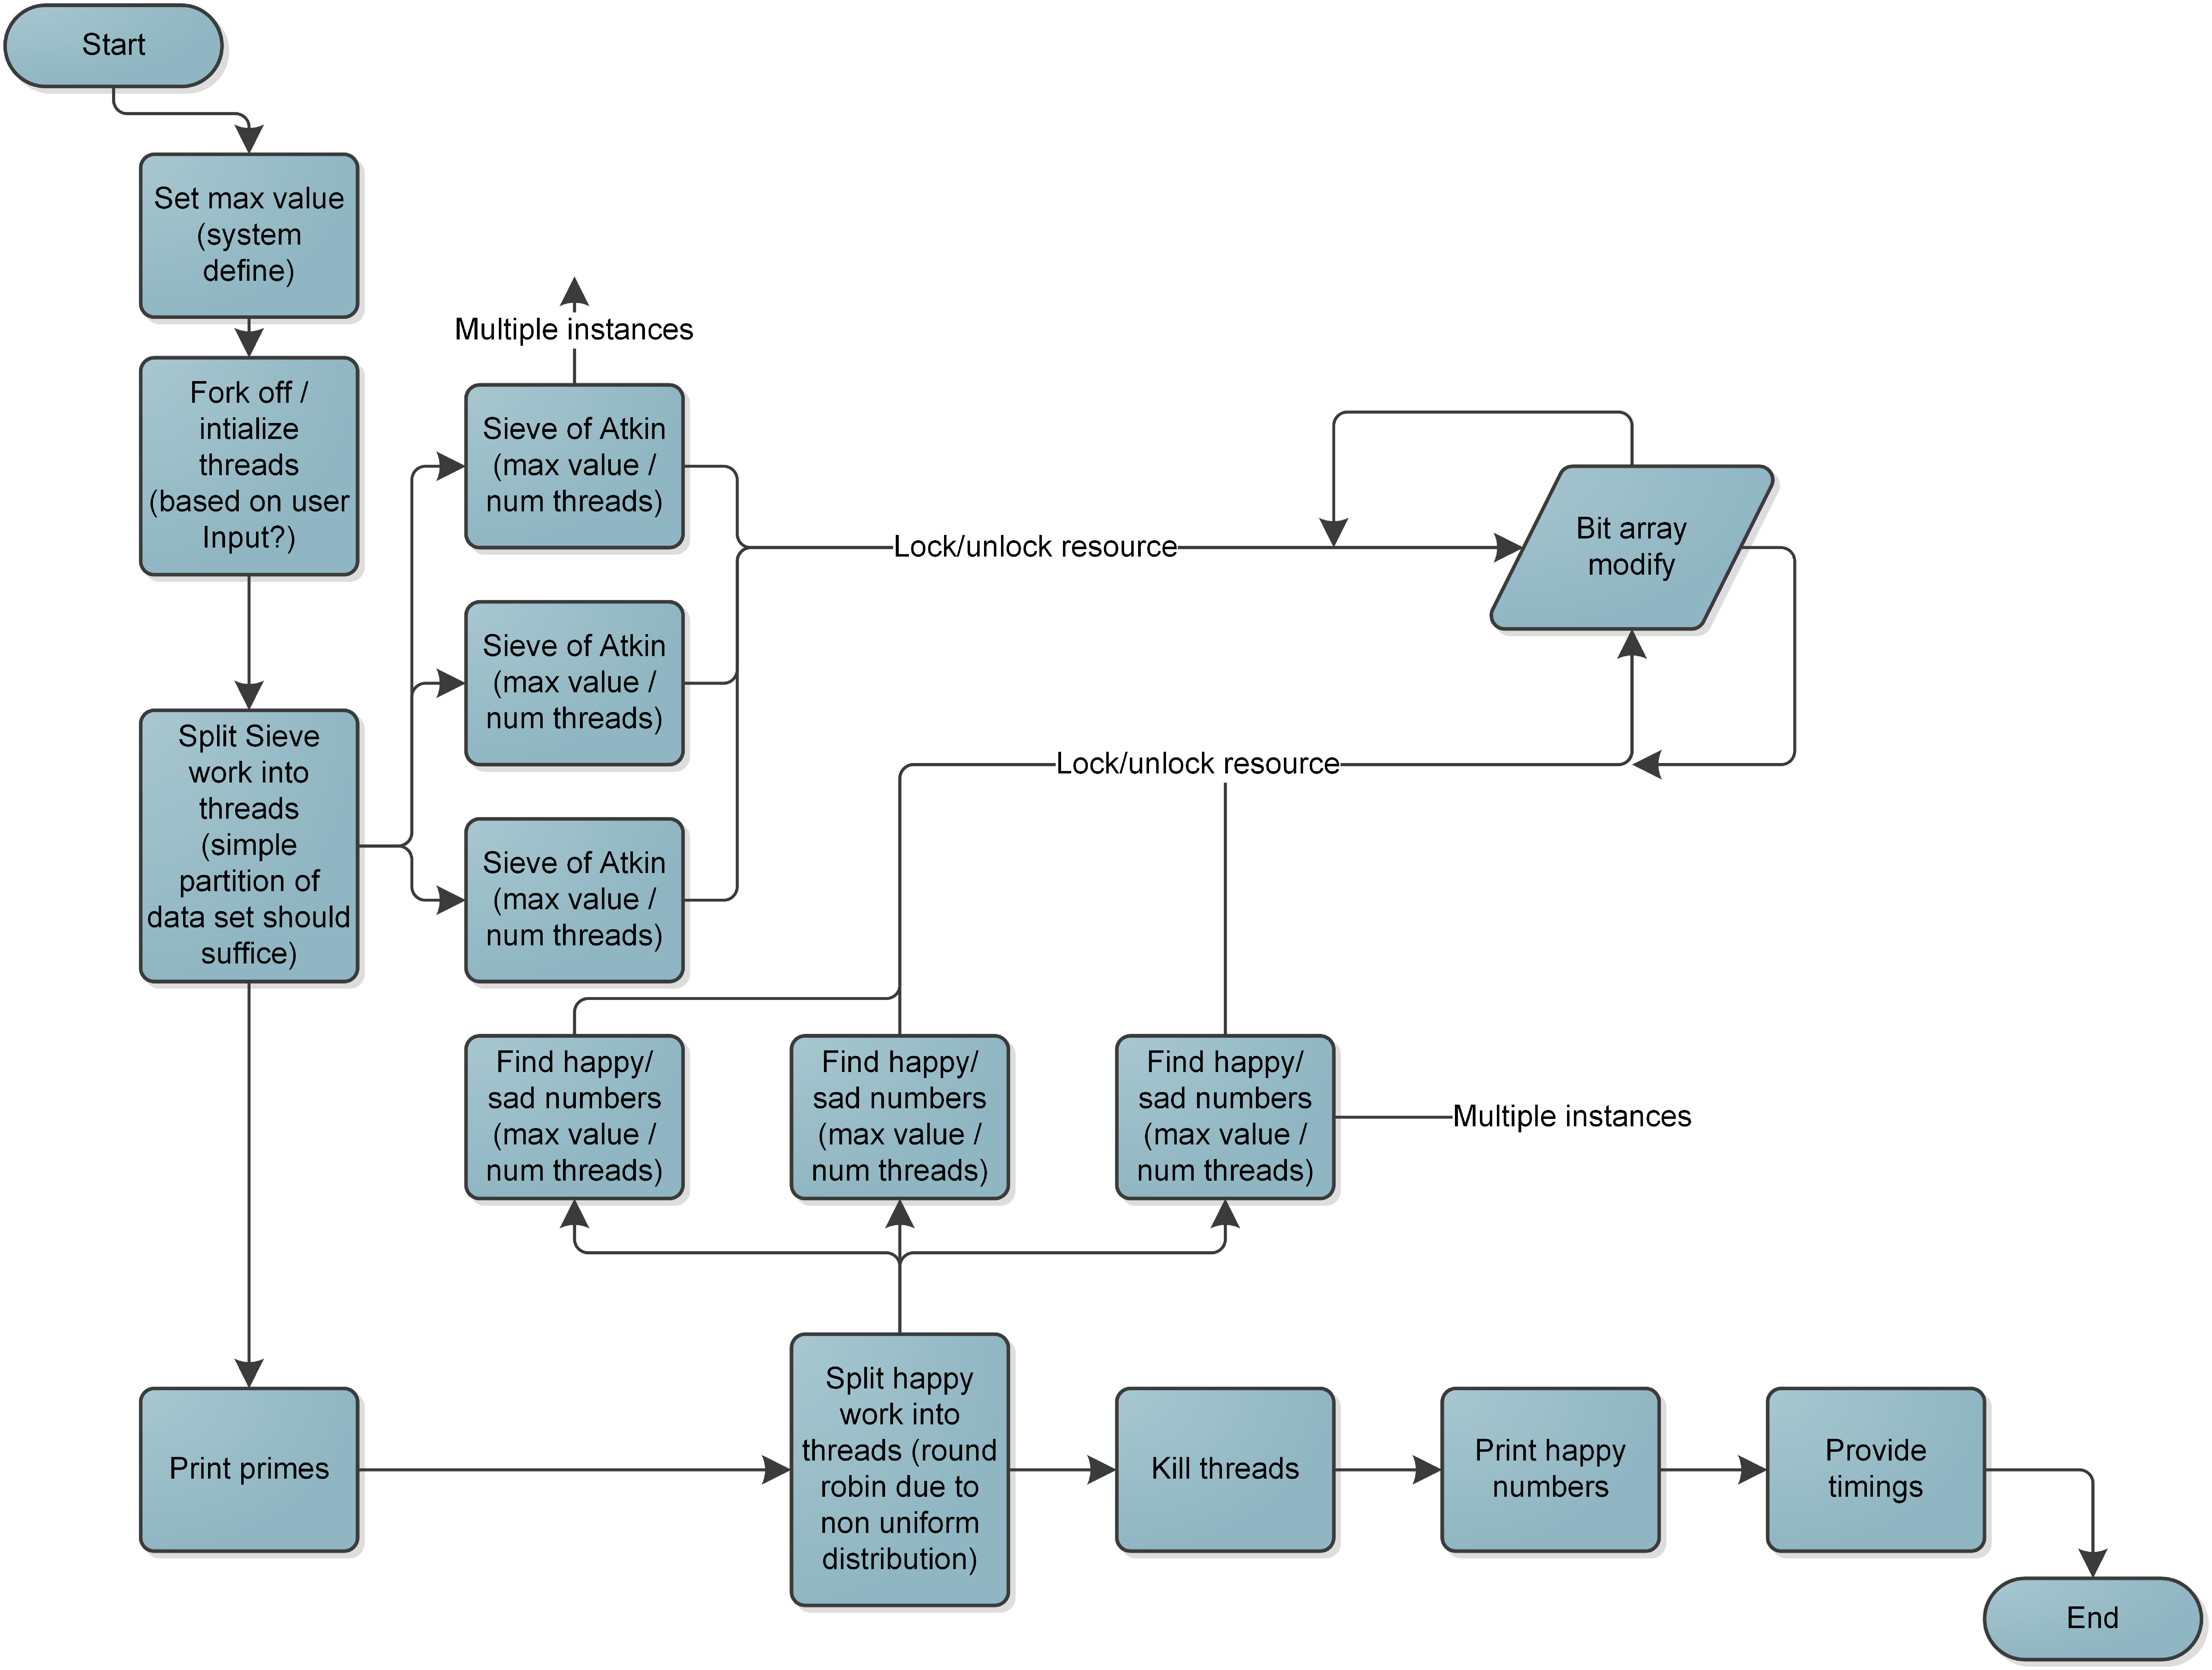
\includegraphics[width=\textwidth]{design.eps}

\section{Work log}
\verbatiminput{git_log.txt}

\section{Timings}

\section{Discussion}
I chose the system design as the simplest capable of meeting all of the program
requirements. One of my largest concerns was getting the prime calculation done
in under 45 seconds. Using serial code, I was able to get the Sieve of Atkin
serialized down to around three minutes (on my personal laptop, with a Core
i3 380M). Then parallelizing this using processes and threads, I was still
unable to beat the 45 second mark. One of the biggest challenges trying to do
so was simply locking the bitmap for thread safe operations, using semaphores
and mutexes. The broad-level implementation was clean, understandable and easy
however most of my speed issues came from lower level details. For example,
using a mutex for each 8 bit bitmap entry was ridiculously space inefficient.
At around 40 bytes each (IIRC), the mutex array was many many times larger, and
caused my 4GB system on Arch Linux to run out of RAM and crap out. On the flip
side, using a single mutex for the entire array with $2^{32} - 1$ entries was
ridiculously slow, and using no locking at all was unacceptable.

The design I came up with was high level enough I didn't expect to make changes.
Unfortunately I did end up respawning threads (I was originally planning on
using a condition variable to sync all of them up) due to project time constrains.
I would like to tweak my code to use a condition variable (and only spawn threads
once) but that has not happened yet.
\end{document}
